\documentclass[a4paper,oneside,14pt]{extarticle}

\usepackage{cmap} % Улучшенный поиск русских слов в полученном pdf-файле
\usepackage[T2A]{fontenc} % Поддержка русских букв
\usepackage[utf8]{inputenc} % Кодировка utf8
\usepackage[english,russian]{babel} % Языки: русский, английский

\usepackage[14pt]{extsizes}

\usepackage{graphicx}
\usepackage{multirow}

\usepackage{tikz}
\usetikzlibrary{shapes, shapes.geometric, arrows, arrows.meta, positioning}

\usepackage{caption}
\captionsetup{labelsep=endash}
\captionsetup[figure]{name={Рисунок}}

\usepackage{amsmath}
\usepackage{amsfonts}

\usepackage{geometry}
\geometry{left=30mm}
\geometry{right=10mm}
\geometry{top=20mm}
\geometry{bottom=20mm}

\usepackage{enumitem}

\usepackage{tabularx}
\usepackage{longtable}
\usepackage{adjustbox}
\usepackage{threeparttable}

% Переопределение стандартных \section, \subsection, \subsubsection по ГОСТу;
\usepackage{titlesec}[explicit]
\titleformat{name=\section,numberless}[block]{\normalfont\large\bfseries\centering}{}{0pt}{}
\titleformat{\section}[block]{\normalfont\large\bfseries}{\thesection}{1em}{}
\titlespacing\section{\parindent}{*4}{*4}

\titleformat{\subsection}[hang]
{\bfseries\large}{\thesubsection}{1em}{}
\titlespacing\subsection{\parindent}{*2}{*2}

\titleformat{\subsubsection}[hang]
{\bfseries\large}{\thesubsubsection}{1em}{}
\titlespacing\subsubsection{\parindent}{*2}{*2}

\usepackage{url}

% Переопределение их отступов до и после для 1.5 интервала во всем документе
\usepackage{setspace}
\onehalfspacing % Полуторный интервал
\frenchspacing
\setlength\parindent{1.25cm}

\usepackage{indentfirst} % Красная строка

% Настройки оглавления
\usepackage{xcolor}
\usepackage{multirow}

% Гиперссылки
\usepackage[pdftex]{hyperref}
\hypersetup{hidelinks}

% Дополнительное окружения для подписей
\usepackage{array}
\newenvironment{signstabular}[1][1]{
	\renewcommand*{\arraystretch}{#1}
	\tabular
}{
	\endtabular
}

\usepackage{enumitem} 
\setenumerate[0]{label=\arabic*)} % Изменение вида нумерации списков
\renewcommand{\labelitemi}{---}

% Листинги 
\usepackage{courier}
\usepackage{listings}
\usepackage{chngcntr} % Listings counter within section set main.tex after begin document
\usepackage{float} % Place figures anywhere you want; ignore floating
\floatstyle{plaintop}
\newfloat{code}{H}{myc}

% Для листинга кода:
\lstset{
	basicstyle=\small\ttfamily,			% размер и начертание шрифта для подсветки кода
	language=C++,   					% выбор языка для подсветки	
	numbers=left,						% где поставить нумерацию строк (слева\справа)
	numbersep=5pt,
	% stepnumber=1,						% размер шага между двумя номерами строк
	xleftmargin=17pt,
	% showstringspaces=false,
	numbersep=5pt,						% как далеко отстоят номера строк от подсвечиваемого кода
	frame=single,						% рисовать рамку вокруг кода
	tabsize=4,							% размер табуляции по умолчанию равен 4 пробелам
	captionpos=b,						% позиция заголовка вверху [t] или внизу [b]
	breaklines=true,					
	breakatwhitespace=true,				% переносить строки только если есть пробел
	escapeinside={\#*}{*)},				% если нужно добавить комментарии в коде
	inputencoding=utf8x,
	backgroundcolor=\color{white},
	numberstyle=,%\tiny,					    % размер шрифта для номеров строк
	keywordstyle=\color{blue},
	stringstyle=\color{red!90!black}, % color of text in ""
	commentstyle=\color{green!50!black}
}
\lstdefinelanguage[RISC-V]{Assembler}
{
  alsoletter={.}, % allow dots in keywords
  alsodigit={0x}, % hex numbers are numbers too!
  morekeywords=[1]{ % instructions
    lb, lh, lw, lbu, lhu,
    sb, sh, sw,
    sll, slli, srl, srli, sra, srai,
    add, addi, sub, lui, auipc,
    xor, xori, or, ori, and, andi,
    slt, slti, sltu, sltiu,
    beq, bne, blt, bge, bltu, bgeu,
    j, jr, jal, jalr, ret,
    scall, break, nop
  },
  morekeywords=[2]{ % sections of our code and other directives
    .align, .ascii, .asciiz, .byte, .data, .double, .extern,
    .float, .globl, .half, .kdata, .ktext, .set, .space, .text, .word
  },
  morekeywords=[3]{ % registers
    zero, ra, sp, gp, tp, s0, fp,
    t0, t1, t2, t3, t4, t5, t6,
    s1, s2, s3, s4, s5, s6, s7, s8, s9, s10, s11,
    a0, a1, a2, a3, a4, a5, a6, a7,
    ft0, ft1, ft2, ft3, ft4, ft5, ft6, ft7,
    fs0, fs1, fs2, fs3, fs4, fs5, fs6, fs7, fs8, fs9, fs10, fs11,
    fa0, fa1, fa2, fa3, fa4, fa5, fa6, fa7
  },
  morecomment=[l]{;},   % mark ; as line comment start
  morecomment=[l]{\#},  % as well as # (even though it is unconventional)
  morestring=[b]",      % mark " as string start/end
  morestring=[b]'       % also mark ' as string start/end
}
\lstset{
	basicstyle=\small\ttfamily,			% размер и начертание шрифта для подсветки кода
    language=[RISC-V]Assembler,   					% выбор языка для подсветки	
	numbers=left,						% где поставить нумерацию строк (слева\справа)
	numbersep=5pt,
	% stepnumber=1,						% размер шага между двумя номерами строк
	xleftmargin=17pt,
	% showstringspaces=false,
	numbersep=5pt,						% как далеко отстоят номера строк от подсвечиваемого кода
	frame=single,						% рисовать рамку вокруг кода
	tabsize=4,							% размер табуляции по умолчанию равен 4 пробелам
	captionpos=b,						% позиция заголовка вверху [t] или внизу [b]
	breaklines=true,					
	breakatwhitespace=true,				% переносить строки только если есть пробел
	escapeinside={\#*}{*)},				% если нужно добавить комментарии в коде
	inputencoding=utf8x,
	backgroundcolor=\color{white},
	numberstyle=,%\tiny,					    % размер шрифта для номеров строк
	keywordstyle=\color{blue},
	stringstyle=\color{red!90!black}, % color of text in ""
	commentstyle=\color{green!50!black}
}
\lstset{
 morekeywords={size_t, likely}
}

\lstset{
	literate=
	{а}{{\selectfont\char224}}1
	{б}{{\selectfont\char225}}1
	{в}{{\selectfont\char226}}1
	{г}{{\selectfont\char227}}1
	{д}{{\selectfont\char228}}1
	{е}{{\selectfont\char229}}1
	{ё}{{\"e}}1
	{ж}{{\selectfont\char230}}1
	{з}{{\selectfont\char231}}1
	{и}{{\selectfont\char232}}1
	{й}{{\selectfont\char233}}1
	{к}{{\selectfont\char234}}1
	{л}{{\selectfont\char235}}1
	{м}{{\selectfont\char236}}1
	{н}{{\selectfont\char237}}1
	{о}{{\selectfont\char238}}1
	{п}{{\selectfont\char239}}1
	{р}{{\selectfont\char240}}1
	{с}{{\selectfont\char241}}1
	{т}{{\selectfont\char242}}1
	{у}{{\selectfont\char243}}1
	{ф}{{\selectfont\char244}}1
	{х}{{\selectfont\char245}}1
	{ц}{{\selectfont\char246}}1
	{ч}{{\selectfont\char247}}1
	{ш}{{\selectfont\char248}}1
	{щ}{{\selectfont\char249}}1
	{ъ}{{\selectfont\char250}}1
	{ы}{{\selectfont\char251}}1
	{ь}{{\selectfont\char252}}1
	{э}{{\selectfont\char253}}1
	{ю}{{\selectfont\char254}}1
	{я}{{\selectfont\char255}}1
	{А}{{\selectfont\char192}}1
	{Б}{{\selectfont\char193}}1
	{В}{{\selectfont\char194}}1
	{Г}{{\selectfont\char195}}1
	{Д}{{\selectfont\char196}}1
	{Е}{{\selectfont\char197}}1
	{Ё}{{\"E}}1
	{Ж}{{\selectfont\char198}}1
	{З}{{\selectfont\char199}}1
	{И}{{\selectfont\char200}}1
	{Й}{{\selectfont\char201}}1
	{К}{{\selectfont\char202}}1
	{Л}{{\selectfont\char203}}1
	{М}{{\selectfont\char204}}1
	{Н}{{\selectfont\char205}}1
	{О}{{\selectfont\char206}}1
	{П}{{\selectfont\char207}}1
	{Р}{{\selectfont\char208}}1
	{С}{{\selectfont\char209}}1
	{Т}{{\selectfont\char210}}1
	{У}{{\selectfont\char211}}1
	{Ф}{{\selectfont\char212}}1
	{Х}{{\selectfont\char213}}1
	{Ц}{{\selectfont\char214}}1
	{Ч}{{\selectfont\char215}}1
	{Ш}{{\selectfont\char216}}1
	{Щ}{{\selectfont\char217}}1
	{Ъ}{{\selectfont\char218}}1
	{Ы}{{\selectfont\char219}}1
	{Ь}{{\selectfont\char220}}1
	{Э}{{\selectfont\char221}}1
	{Ю}{{\selectfont\char222}}1
	{Я}{{\selectfont\char223}}1
}

% Работа с изображениями и таблицами; переопределение названий по ГОСТу
\usepackage{caption}
\captionsetup[figure]{name={Рисунок},labelsep=endash}
\captionsetup[table]{singlelinecheck=false, labelsep=endash}

\usepackage[justification=centering]{caption} % Настройка подписей float объектов	

\usepackage{csvsimple}

\usepackage{ulem} % Нормальное нижнее подчеркивание
\usepackage{hhline} % Двойная горизонтальная линия в таблицах
\usepackage[figure,table]{totalcount} % Подсчет изображений, таблиц
\usepackage{rotating} % Поворот изображения вместе с названием
\usepackage{lastpage} % Для подсчета числа страниц

\makeatletter
\renewcommand\@biblabel[1]{#1.} % [1] -> 1. in bibliography
\makeatother

\usepackage{ragged2e} % Перенос слов на следующую строку
\usepackage{pdfpages}

\usepackage{blindtext}

% \usepackage[
%     backend=biber,
% 	style=gost-numeric,
% 	% style=numeric-comp,
% 	language=auto,
% 	autolang=other,
% 	sorting=none
% ]{biblatex}
% \addbibresource{bibliography.bib}
% \usepackage{xparse} % \NewDocumentCommand for creating custom commands
% \NewDocumentCommand{\printbib}{m}
% {\printbibliography[title={#1}]\addcontentsline{toc}{section}{#1}}


\begin{document}

\def\coursename{Анализ Алгоритмов}
\def\labnumber{\textbf{\textcolor{red}{X}}}
\def\labtheme{\textbf{\textcolor{red}{Тема}}}
\def\myname{Рунов К.А.}
\def\mygroup{ИУ7-54Б}
\def\teachers{Волкова Л. Л., Строганов Д. В.}

\begin{titlepage}
    \newgeometry{left=2cm, right=1cm, top=2.5cm, bottom=2.5cm}
    \fontsize{12pt}{12pt}\selectfont

    \noindent
    \begin{center}
        % \fbox
        % \begin{tabular}{|l|r|}
        % {
            % \hline
            \begin{minipage}{0.12\textwidth}
                
\includegraphics[width=\linewidth]{img/bmstu_logo.jpg}
            \end{minipage}
            \hfill
            % &
            % \hspace{0.2cm}
            \begin{minipage}{0.85\textwidth}\centering\bfseries
                {
                    \linespread{1}\selectfont
                    \vspace{0.1cm}
                    % \textsc
                    {Министерство науки и высшего образования~Российской~Федерации}

                    % \textsc
                    {Федеральное~государственное~бюджетное~образовательное~учреждение высшего образования}

                    % \textsc
                    {<<Московский государственный технический университет имени~Н.~Э.~Баумана (национальный~исследовательский~университет)>>}

                    % \textsc
                    {(МГТУ им. Н.~Э.~Баумана)}
                    \vspace{0.1cm}
                }
            \end{minipage}
            % \\
            % \hline
        % }
        % \end{tabular}

        \vspace{0.2cm}
        \rule{\linewidth}{2.8pt}
        \rule[3ex]{\linewidth}{1pt}

        \begin{flushleft}
            {ФАКУЛЬТЕТ \uline{<<Информатика и системы управления>> \hfill}}

            \vspace{0.5cm}

            {КАФЕДРА \uline{<<Программное обеспечение ЭВМ и информационные технологии>> \hfill}}
        \end{flushleft}

        % \vspace{1cm}
        \vfill

        {
            \Large{\textbf{
                % \bolduline
                {ОТЧЕТ ПО ЛАБОРАТОРНОЙ РАБОТЕ №\labnumber}
            }}

            \Large{\textbf{
                % \bolduline
                {по курсу <<\coursename>>}
            }}

            \Large{\textbf{
                % \bolduline
                {на тему:}
            }}

            \large{<<\labtheme>>}

            \vspace{0.5cm}
        }

        \vspace{0.5cm}

        % \setstretch{1.5}
        % \begin{tabular}{p{\textwidth}}
        %     \uline
        %     {
        %         Разработка программы для моделирования столкновений объектов
        %         в виртуальном пространстве. \hfill
        %     }
        %     \rule{\linewidth}{0.4pt}
        % \end{tabular}

        \fontsize{14pt}{14pt}\selectfont

        % \vfill

        \begin{flushleft}
            % {Студент \uline{Рунов Константин Алексеевич \hfill}}
            {Студент \uline{\myname \hfill}}

            \vspace{0.5cm}

            {Группа \uline{\mygroup \hfill}}

            \vspace{0.5cm}

            % {Оценка (баллы) \uline{\hfill}}

            % \vspace{0.5cm}

            % {Преподаватель \hfill \ulinetext[4cm]{(Подпись, дата)}{} \ulinetext[4cm]{}{Волкова Л.~Л.}}
            % {Преподаватели \uline{Волкова Лилия Леонидовна, Строганов Дмитрий Владимирович \hfill}}
            {Преподаватели \uline{\teachers \hfill}}

            % \vspace{0.5cm}

            % {Преподаватель \hfill \ulinetext[4cm]{(Подпись, дата)}{} \ulinetext[4cm]{}{Строганов Д.~В.}}

            \vspace{0.5cm}

        \end{flushleft}

        \vfill

        \the\year\ г.

    \end{center}
\end{titlepage}


\setcounter{page}{2}
\renewcommand{\contentsname}{СОДЕРЖАНИЕ}
\tableofcontents

\newpage

\section{Функции обработчика прерывания от системного таймера}

\subsection{Windows}

\subsubsection{По тику}
\begin{itemize}
	\item инкремент счетчика системного времени;
	\item декремент кванта текущего потока;
	\item декремент счетчиков времени отложенных задач;
    \item если активен механизм профилирования ядра, то инициализация отложенного вызова обработчика ловушки профилирования ядра добавлением объекта в очередь DPC (обработчик ловушки профилирования регистрирует адрес команды, выполнявшейся на момент прерывания);
	\item инкремент часов и прочих системных таймеров.
\end{itemize}

\subsubsection{По главному тику}
\begin{itemize}
    \item освобождение объекта <<событие>>, на котором ожидает диспетчет настройки баланса (диспетчер настройки баланса по событию от таймера сканирует очередь готовых процессов и повышает приоритет процессов, которые находились в очереди в состоянии ожидания дольше 4х секунд \cite[с.~511]{windows}).
\end{itemize}

\subsubsection{По кванту}
\begin{itemize}
    \item инициация диспетчеризации потоков добавлением соответствующего объекта в очередь DPC \cite[c.~146]{windows}.
\end{itemize}

\subsection{UNIX}

\subsubsection{По тику}
\begin{itemize}
	\item инкремент счетчика тиков аппаратного таймера;
	\item инкремент часов и других таймеров системы;
	\item обновление статистики использования процессора текущим процессом (инкрементмент поля p\_cpu дескриптора текущего процесса до максимального значения, равного 127);
	\item декремент счетчика времени, оставшегося до отправления на выполнение отложенных вызовов, при достижении нулевого значения счетчика --- выставление флага, указывающего на необходимость запуска обработчика отложенного вызова;
    \item декремент кванта.
\end{itemize}

\subsubsection{По главному тику} 
\begin{itemize}
	\item регистрация отложенных вызовов функций, относящихся к работе планировщика,
	таких как пересчет приоритетов;
	\item пробуждение (то есть регистрирация отложенного вызова процедуры wakeup, которая перемещает дескриптор процесса из списка <<спящих>> в очередь <<готовых к выполнению>>) системных процессов swapper и pagedaemon;
	\item декремент счетчика времени, оставшегося до посылки одного из следующих сигналов:
	\begin{itemize}
		\item SIGALRM --- сигнал, посылаемый процессу по истечении времени, заданного функцией alarm() (будильник реального времени);
		\item SIGPROF --- сигнал, посылаемый процессу по истечении времени, заданного в таймере профилирования (будильник профиля процесса);
		\item SIGVTALRM --- сигнал, посылаемый процессу по истечении времени работы в режиме задачи (будильник виртуального времени).
	\end{itemize}
\end{itemize}

\subsubsection{По кванту}
\begin{itemize}
	\item если текущий процесс превысил выделенный ему квант процессорного времени, отправка ему сигнала SIGXCPU \cite[c.~188]{unix} \cite[c.~257]{unixrob}.
\end{itemize}

\section{Пересчет динамических приоритетов}

Динамические приоритеты могут быть только у пользовательских процессов. В операционных системах процесс является владельцем ресурсов, в том числе --- владельцем приоритета.

\subsection{Windows}
%475 Р
В Windows реализуется приоритетная, вытесняющая система планирования, при  которой всегда выполняется хотя бы один работоспособный (готовый) поток с самым высоким приоритетом. 

После того как поток был выбран для запуска, он запускается на время, называемое квантом.
Но поток может и не израсходовать свой квант времени: если становится готов к запуску другой поток с более высоким приоритетом, текущий выполняемый поток может быть вытеснен.

Единого модуля под названием «планировщик» не существует.
Процедуры, выполняющие обязанности по диспетчеризации, обобщенно называются диспетчером ядра.
Диспетчеризации потоков могут потребовать следующие события:
\begin{itemize}
	\item поток становится готовым к выполнению;
	\item поток выходит из состояния выполнения из-за окончания его кванта времени;
	\item поток завершается или переходит в состояние ожидания;
	\item изменяется приоритет потока;
	\item изменяется родственность процессора потока.
\end{itemize}

Windows использует 32 уровня приоритета, от 0 до 31. Эти значения  разбиваются на части следующим образом:
\begin{itemize}
	\item шестнадцать уровней реального времени (от 16 до 31);
	\item шестнадцать изменяющихся уровней (от 0 до 15), из которых уровень 0 зарезервирован для потока обнуления страниц. 
\end{itemize}

Уровни приоритета потоков назначаются из двух разных позиций: от Windows API и от ядра Windows \cite[c.~478]{windows}.

Windows API систематизирует процессы по классу приоритета, который присваивается им при их создании:
\begin{itemize}
	\item реального времени (real-time (4));
	\item высокий (high (3));
	\item выше обычного (above normal (7));
	\item обычный (normal (2));
	\item ниже обычного (below normal (5));
	\item простой (idle (1)).
\end{itemize}

Затем назначается относительный приоритет потоков в рамках процессов.
Здесь номера представляют изменение приоритета, применяющееся к базовому приоритету процесса:
\begin{itemize}
	\item критичный по времени (time-critical (15));
	\item наивысший (highest (2));
	\item выше обычного (above normal (1));
	\item обычный (normal (0));
	\item ниже обычного (below normal (-1));
	\item самый низший (lowest (-2));
	\item простоя (idle (-15)).
\end{itemize}

Уровень, критичный по времени, и уровень простоя (+15 и -15) называются уровнями насыщения и представляют конкретные применяемые уровни вместо смещений.
Относительный приоритет --- это приращение к базовому приоритету процесса.

Соответствие между приоритетами Windows API и ядра Windows приведено в таблице \ref{tbl:priority}.
\begin{table}[h]
    \caption{Соответствие между приоритетами Windows API и ядра Windows \cite[c.~479]{windows}}
	\begin{center}
		\begin{tabular}{|l|p{45pt}|p{45pt}|p{45pt}|p{45pt}|p{45pt}|p{45pt}|} 
			\hline
			{} & {real-time} & {high} & {above normal} & {normal} & {below normal} & {idle}\\
			\hline
			{time critical} & 31 & 15 & 15 & 15 & 15 & 15 \\
			\hline
			{highest} & 26 & 15 & 12 & 10 & 8 & 6 \\
			\hline
			{above normal} & 25 & 14 & 11 & 9 & 7 & 5 \\
			\hline
			{normal} & 24 & 13 & 10 & 8 & 6 & 4 \\
			\hline
			{below normal} & 23 & 12 & 9 & 7 & 5 & 3 \\
			\hline
			{lowest} & 22 & 11 & 8 & 6 & 4 & 2 \\
			\hline
			{idle} & 16 & 1 & 1 & 1 & 1 & 1 \\
			\hline
		\end{tabular}
	\end{center}
	\label{tbl:priority}
\end{table}

Приложения пользователя обычно запускаются с базовым приоритетом (normal), поэтому их исходный поток чаще всего выполняется с уровнем приоритета 8. 

У процесса имеется только одно базовое значение приоритета, а у каждого потока имеется два значения приоритета: текущее (динамическое) и базовое.
Решения по планированию принимаются исходя из текущего приоритета.
Система при определенных обстоятельствах на короткие периоды времени повышает приоритет потоков в динамическом диапазоне (от 1 до 15).
Windows никогда не регулирует приоритет потоков в диапазоне реального времени (от 16 до 31), поэтому они всегда имеют один и тот же базовый и текущий приоритет.

Исходный базовый приоритет потока наследуется от базового приоритета процесса.
Процесс по умолчанию наследует свой базовый приоритет у того процесса, который его создал.

Планировщик Windows периодически настраивает текущий приоритет потоков, используя внутренний механизм повышения приоритета.
Во многих случаях это делается для уменьшения различных задержек и повышения восприимчивости системы, а также чтобы у потоков была возможность выполнения и освобождения ресурсов.  


Повышение приоритета вступает в действие немедленно и может  вызвать изменения в планировании процессора.
Однако если поток использует весь свой следующий квант, то он теряет один уровень приоритета.
Если же он использует второй полный квант, то он перемещается вниз еще  на один уровень, и так до тех пор, пока не дойдет до своего базового уровня. 

Сценарии повышения приоритета:
\begin{itemize}
	\item Повышение вследствие событий планировщика или диспетчера (сокращение задержек).
	\item Повышение вследствие завершения ввода-вывода (сокращение задержек --- поток может вновь запуститься и начать новую операцию ввода-вывода). В таблице \ref{tab:io} приведены рекомендуемые значения повышения приоритета для устройств ввода-вывода.
	\item Повышение вследствие ввода из пользовательского интерфейса (сокращение задержек и времени отклика).
	\item Повышение приоритета владельца блокировки.
	\item Повышение вследствие слишком продолжительного ожидания ресурса исполняющей системы (предотвращение зависания).
	\item Повышение в случае, когда готовый к запуску поток не был запущен в течение определенного времени (чтобы исключить бесконечное откладывание процессов).
	%табличку
	%\item Если поток ждал на семафоре, мьютексе или другом событии, то повышение при его освобождении.
	\item Повышение вследствие ожидания объекта ядра.
	\item Повышение приоритета потоков первого плана после ожидания (улучшение отзывчивости интерактивных приложений).
	\item Повышение приоритета после пробуждения GUI-потока (потоки-владельцы окон получают при пробуждении дополнительное повышение приоритета на 2).
	\item Повышения приоритета, связанные с перезагруженностью центрального процессора (CPU Starvation).
	\item Другие псевдоповышающие механизмы, проявляющие себя при проигрывании мультимедиа. В отличие от других повышений приоритета, эти механизмы применяются непосредственно в режиме ядра. Повышение приоритета проигрывания мультимедиа управлятся службой планировщика класса мультимедиа MMCSS (это не является настоящим повышением, служба просто устанавливает по необходимости новые базовые приоритеты для потоков).
\end{itemize}

\begin{table}[h!]
	\caption{Рекомендуемые значения повышения приоритета.}
	\begin{center}
		\begin{tabular}{|p{100mm}|l|}
			\hline
			{Устройство} & {Приращение} \\
			\hline
			Жесткий диск, привод компакт-дисков, параллельный порт, видеоустройство & 1 \\
			\hline
			Сеть, почтовый слот, именованный канал, последовательный порт & 2 \\
			\hline
			Клавиатура, мышь & 6 \\
			\hline
			Звуковое устройство & 8 \\
			\hline
		\end{tabular}
	\end{center}
	\label{tab:io}
\end{table}

Рассмотрим последние 2 сценария подробней. 

% \textbf{Перезагруженность центрального процессора}
% \subsection*{Перезагруженность центрального процессора}

% В Windows включен общий механизм ослабления загруженности центрального процессора, который называется диспетчером настройки баланса и является частью системного потока.

% Один раз в секунду этот поток сканирует очередь готовых потоков в поиске тех из них, которые находятся в состоянии ожидания около 4 секунд.
% Если такой поток будет найден, диспетчер настройки баланса повышает его приоритет до 15 единиц и устанавливает квантовую цель эквивалентной тактовой частоте процессора при подсчете 3 квантовых единиц.
% Как только квант истекает, приоритет потока тут же снижается до обычного базового приоритета.
% Если поток не был завершен и есть готовый к запуску поток с более высоким уровнем приоритета, поток с пониженным приоритетом возвращается в очередь готовых потоков.

% Для минимизации времени своей работы, диспетчер настройки баланса сканирует только 16 готовых потоков.
% Если на данном уровне приоритета имеется больше потоков, он запоминает то место, на котором остановился, и начинает с него при следующем проходе очереди.
% Кроме того, он за один проход повысит приоритет только 10 потоков.
% Если найдет 10 потоков, заслуживающих именно этого повышения, он прекратит сканирование на этом месте и начнет его с этого же места при следующем проходе.

% \textbf{MMCSS}
\subsection*{MMCSS}

MMCSS работает с вполне определенными задачами, включая следующие: аудио, захват, распределение, игры, проигрывание, аудио профессионального качества, задачи администратора многооконного режима.

Каждая из этих задач включает информацию о свойствах, отличающих их друг от друга.
Одно из наиболее важных свойств для планирования потоков называется категорией планирования --- Scheduling Category, которое является первичным фактором, определяющим приоритет потоков, зарегистрированных с MMCSS.
На рисунке \ref{img:6} показаны различные категории планирования.

\begin{figure}[h]
	\centering
	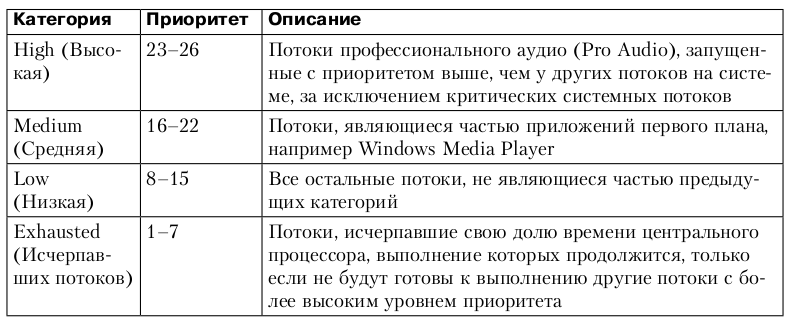
\includegraphics[width=0.9\textwidth]{img/6.png}
    \caption{Категории планирования \cite[c.~518]{windows}}
	\label{img:6}
\end{figure}

Механизм, положенный в основу MMCSS, повышает приоритет потоков внутри зарегистрированного процесса до уровня, соответствующего их категории планирования и относительного приоритета внутри этой категории на гарантированный срок.
Затем он снижает категорию этих потоков до Exhausted, чтобы другие, не относящиеся к мультимедийным приложениям потоки, также могли получить ресурс.

\subsection{UNIX}

В современных системах UNIX ядро является вытесняющим --- процесс в режиме ядра может быть вытеснен более приоритетным процессом, также находящимся в режиме ядра.
Это сделано для того, чтобы система могла обслуживать процессы реального времени, такие как  аудио и видео.

Согласно приоритетам процессов и принципу вытесняющего циклического планирования формируется очередь готовых к выполнению процессов.
В первую очередь выполняются процессы с большим приоритетом.
Процессы с одинаковыми приоритетами выполняются в течении кванта времени, циклически друг за другом.

Приоритет задается любым целым числом, лежащим в диапазоне от 0 до 127 (чем меньше число, тем выше приоритет).
Приоритеты от 0 до 49 зарезервированы для ядра, они являются фиксированными величинами.
Прикладные процессы могут обладать приоритетом в диапазоне 50~--~127.

В традиционных системах UNIX приоритет процесса определяется двумя факторами: 
\begin{itemize}
	\item фактор <<любезности>> – целое число в диапазоне от 0 до 39 со значением 20 по умолчанию. Чем меньше значение фактора любезности, тем выше приоритет процесса. Пользователи могут повлиять на приоритет процесса при помощи изменения этого фактора, используя системный вызов nice (но только суперпользователь имеет полномочия увеличивать приоритет процесса);
	\item фактор утилизации --- степень загруженности CPU в момент последнего обслуживания им процесса. Этот фактор позволяет системе динамически изменять приоритет процесса.
\end{itemize}

Планировщик использует p\_pri для принятия решения о том, какой процесс направить на выполнение.
У процесса, находящегося в режиме задачи, значения p\_pri и p\_usrpri идентичны.
Значение текущего приоритета p\_pri может быть повышено планировщиком для выполнения процесса в режиме ядра.
Когда процесс просыпается после блокировки в системном вызове, его приоритет временно повышается.
При создании процесса поле p\_cpu инициализируется нулем.
На каждом тике обработчик таймера увеличивает поле p\_cpu текущего процесса на единицу, до максимального значения, равного 127 \cite[c.~194]{unix}.

% NOTE: хз, откуда, но в интернете есть по запросу "приоритеты ядра"
\newpage
\begin{table}[h]
    \caption{Таблица приоритетов в системе 4.3BSD UNIX}
	\label{tab:bsd}
	\begin{center}
		\begin{tabular}{ |c|c|c|  }
			\hline
			{Приоритет} & {Значение} & {Описание} \\
			\hline
			{PSWP} & 0 & Свопинг \\
			\hline
			{PSWP + 1} & 1 & Страничный демон \\
			\hline
			{PSWP + 1/2/4} & 1/2/4 & Другие действия по обработке памяти \\
			\hline
			{PINOD} & 10 & Ожидание освобождения inode \\
			\hline
			{PRIBIO} & 20 & Ожидание дискового ввода-вывода \\
			\hline
			{PRIBIO + 1} & 21 & Ожидание освобождения буфера \\
			\hline
			{PZERO} & 25 & Базовый приоритет \\
			\hline
			{TTIPRI} & 28 & Ожидание ввода с терминала \\
			\hline
			{TTOPRI} & 29 & Ожидание вывода с терминала \\
			\hline 
			{PWAIT} & 30 & Ожидание завершения процесса потомка \\
			\hline
			{PLOCK} & 35 & Консультативное ожидание блокир. ресурса \\
			\hline
			{PSLEP} & 40 & Ожидание сигнала \\
			\hline
		\end{tabular}
	\end{center}
\end{table}

\begin{table}[h]
    \caption{Системные приоритеты сна в системах 4.3BSD UNIX и SCO UNIX \cite[c.~263]{unixrob}}
	\begin{center}
		\begin{tabular}{|l|p{75pt}|p{75pt}|} 
			\hline
			{Событие} & {Приоритет 4.3BSD UNIX} & {Приоритет SCO UNIX}\\
			\hline
			{Ожидание загрузки страницы/сегмента} & 0 & 95\\
			\hline
			{Ожидание индексного дескриптора} & 10 & 88\\
			\hline
			{Ожидание ввода/вывода} & 20 & 81 \\
			\hline
			{Ожидание буфера} & 30 & 80\\
			\hline
			{Ожидание терминального ввода} &    & 75\\
			\hline
			{Ожидание терминального вывода} &    & 74\\
			\hline
			{Ожидание завершения выполнения} &    & 73\\
			\hline
			{Ожидание события} & 40 & 66\\
			\hline
		\end{tabular}
	\end{center}
	\label{tbl:sleeppriority}
\end{table}

Каждую секунду обработчик прерывания таймера инициализирует отложенный вызов процедуры schedcpu(), которая уменьшает значение p{\_}cpu каждого процесса исходя из фактора <<полураспада>> (decay factor).
В {\ttfamily 4.3BSD} для расчета полураспада применяется следующая формула:
\[
d = \frac{2\cdot load{\_}average}{2\cdot load{\_}average + 1},
\]
где load{\_}average --- это среднее количество процессов в состоянии готовности к выполнению, за последнюю секунду.
Процедура schedcpu() также пересчитывает приоритеты режима задачи всех процессов по формуле
\[
{p\_usrpri} = PUSER + \frac{p{\_}cpu}{4} + 2\cdot {p{\_}nice},
\]
где {\ttfamily PUSER} --- базовый приоритет в режиме задачи, равный 50 \cite[c.~196]{unix}.

Таким образом, если процесс до вытеснения другим процессом использовал большое количество процессорного времени, его p{\_}cpu будет увеличен, что приведет к увеличению значения p{\_}usrpri и, следовательно, к понижению приоритета.
Чем дольше процесс простаивает в очереди на выполнение, тем меньше его p{\_}cpu, и, соответственно, выше приоритет. 

Такая схема позволяет исключить бесконечное откладывание низкоприоритетных процессов.
При ее применении процессы, которые осуществляют много операций ввода-вывода, получают преимущество, так как они проводят много времени в ожидании завершения этих операций.
Напротив, те процессы, что производят много вычислений, используют большое количество процессорного времени, и их приоритет после вытеснения будет понижен. 

\newpage

\subsection*{Вывод}

% Семейство ОС Windows и семейство OC UNIX оба являются системами разделения времени с динамическими приоритетами и вытеснением.
% В связи с общим подходом обработчик прерывания от системного таймера выполняет в этих системах схожие функции: 

% \begin{itemize}
% 	\item инициализурует отложенные вызовы функций, относящихся к работе планировщика (например, пересчет динамических приоритетов);
% 	\item декрементирует счетчики времени: часов, таймеров, будильников реального времени, а также счетчики времени отложенных действий;
% 	\item выполняет декремент кванта.
% \end{itemize}

% Так как обработчик прерывания таймера выполняется на высочайшем уровне привилегий, и никакая другая работа в системе не может выполняться, пока он не завершится, его работа устроена так, чтобы он выполнялся как можно быстрее. 

% Для того чтобы исключить бесконечное откладывание пользовательских процессов, повысить уровень отзывчивости системы и поддерживать процессы реального времени, такие как аудио и видео, в семействах ОС Windows и UNIX выполняется пересчет их динамических приоритетов, однако реализация пересчета в этих семействах отличается. 

Операционные системы семейств Windows и UNIX являются системами разделения времени с динамическими приоритетами и вытеснением, поэтому обработчик прерывания от системного таймера выполняет в этих системах схожие функции: 
\begin{itemize}
	\item инициализурует отложенные вызовы функций, относящихся к работе планировщика (например, пересчет динамических приоритетов);
	\item инкременитирует счетчики времени и декрементирует счетчики таймеров, будильников реального времени, счетчики времени отложенных задач;
	\item выполняет декремент кванта.
\end{itemize}

Так как обработчик прерывания таймера выполняется на высочайшем уровне привилегий, и никакая другая работа в системе не может выполняться, пока он не завершится, его работа устроена так, чтобы он выполнялся как можно быстрее. 

Для того чтобы исключить бесконечное откладывание пользовательских процессов, повысить уровень отзывчивости системы и поддерживать процессы реального времени, такие как аудио и видео, в семействах ОС Windows и UNIX выполняется пересчет их динамических приоритетов, однако реализация пересчета в этих семействах отличается. 

\newpage

\renewcommand\refname{СПИСОК ИСПОЛЬЗОВАННЫХ ИСТОЧНИКОВ}
\phantomsection\begingroup
\bibliographystyle{modified-utf8gost705u}
\raggedright
\bibliography{bibliography}
\addcontentsline{toc}{section}{СПИСОК ИСПОЛЬЗОВАННЫХ ИСТОЧНИКОВ}
\endgroup

\end{document}
